\documentclass[11pt]{article}
\usepackage{amsmath, amssymb, physics, mathtools, bm}
\usepackage{tikz, pgfplots}
\pgfplotsset{compat=1.18}
\usepackage[margin=2.3cm]{geometry}
\usepackage{siunitx, booktabs, hyperref}
\usepackage{braket}

\newcommand{\D}{\mathrm{D}}
\newcommand{\de}{\mathrm{d}}
\newcommand{\pd}[2]{\frac{\partial #1}{\partial #2}}
\newcommand{\pdd}[2]{\frac{\partial^{2} #1}{\partial #2^{2}}}
\newcommand{\Lap}{\nabla^{2}}

\title{B3 Atomic and Laser Physics, 2021 --- Model Solutions}
\author{}
\date{}

\begin{document}
\maketitle

%==========================================================
\section*{Question 1 --- Zeeman, axial quadrupole and orbital quenching}

\textbf{Problem.} $\bm\mu=-\mu_B\bm L-g_s\mu_B\bm S$, $H_{ZE}=-\bm\mu\cdot\bm B$. (a) Field at which $H_{ZE}$ is a perturbation of fine structure in H. (b) Land\'e $g_J$ for $g_s\!\approx\!2$. (c) H in $V_{\rm ext}=\alpha(x^2+y^2)+\beta z^2$, $\beta=-\alpha/2$, $0<\alpha\ll e^2/4\pi\epsilon_0 a_0^3$: lowest five levels and value of $\beta$ leaving the ground state unmodified. (d) Add weak $\bm B\parallel\hat z$ and $\bm B\parallel\hat x$.

\subsection*{(a) Field for Zeeman $\ll$ fine structure}

Hydrogen fine-structure scale at $n=2$:
\[
\Delta E_{\rm fs}\sim \tfrac{\alpha^2}{16}|E_1|=\tfrac{(1/137)^2}{16}\cdot\SI{13.6}{eV}\simeq\SI{4.5e-5}{eV}.
\]
Demand $\mu_B B\ll\Delta E_{\rm fs}$:
\[
B\ll\frac{\Delta E_{\rm fs}}{\mu_B}=\frac{\SI{4.5e-5}{eV}}{\SI{5.79e-5}{eV/T}}.
\]
Evaluate:
\begin{equation}
\boxed{\;B\lesssim\SI{0.8}{T}\sim\mathcal O(1)\,\si{T}.\;}
\label{eq:Bcrit}
\end{equation}
Above this: Paschen--Back; $\bm L,\bm S$ decouple.

\subsection*{(b) Anomalous Zeeman and Land\'e $g_J$}

Take $\bm B=B\hat z$:
\[
H_{ZE}=\mu_B B(\hat L_z+g_s\hat S_z).
\]
Project $\bm L+g_s\bm S$ onto $\bm J$ (Wigner--Eckart, fixed $J$):
\[
\Braket{(\bm L+g_s\bm S)_z}_{JM_J}=\frac{\Braket{(\bm L+g_s\bm S)\cdot\bm J}}{J(J+1)\hbar^2}M_J\hbar.
\]
Use $\bm L\cdot\bm J=\tfrac12(\bm J^2+\bm L^2-\bm S^2)$, $\bm S\cdot\bm J=\tfrac12(\bm J^2+\bm S^2-\bm L^2)$:
\[
\Braket{(\bm L+g_s\bm S)\cdot\bm J}=\tfrac{\hbar^2}{2}\bigl[(1+g_s)J(J+1)+(1-g_s)\{L(L+1)-S(S+1)\}\bigr].
\]
Read off:
\[
E_{ZE}=g_J\mu_B B M_J,\qquad g_J=\tfrac{1+g_s}{2}+\tfrac{1-g_s}{2}\,\tfrac{L(L+1)-S(S+1)}{J(J+1)}.
\]
Set $g_s=2$:
\begin{equation}
\boxed{\;g_J=1+\frac{J(J+1)+S(S+1)-L(L+1)}{2J(J+1)}.\;}
\label{eq:gJ}
\end{equation}
Each $J$-multiplet splits into $2J+1$ sublevels, spacing $g_J\mu_B B$.

\subsection*{(c) Hydrogen in the axial quadrupole}

Spherical form, $z=r\cos\theta$, $x^2+y^2=r^2\sin^2\theta$:
\[
V_{\rm ext}=\alpha r^2\sin^2\theta+\beta r^2\cos^2\theta.
\]
Insert $\beta=-\alpha/2$, use $\sin^2=1-\cos^2$:
\[
V_{\rm ext}=\alpha r^2-\tfrac{3\alpha}{2}r^2\cos^2\theta=\alpha r^2\bigl(1-\tfrac32\cos^2\theta\bigr).
\]
Apply $P_2(\cos\theta)=\tfrac12(3\cos^2\theta-1)$:
\begin{equation}
V_{\rm ext}=\tfrac{\alpha r^2}{2}-\alpha r^2 P_2(\cos\theta).
\label{eq:Vext}
\end{equation}
Isotropic part shifts every state by $\tfrac\alpha2\Braket{r^2}$; anisotropic part has selection rules $\Delta m=0$, $\Delta\ell=0,\pm 2$ (parity even).

\paragraph{Ground state ($1s$).} $\ell=0$, $\Braket{P_2}=0$:
\[
\Delta E_{1s}=\tfrac{\alpha}{2}\Braket{r^2}_{1s}=\tfrac{\alpha}{2}\cdot 3a_0^2=\tfrac{3\alpha a_0^2}{2}.
\]

\paragraph{$n=2$ shell.} $r^2$ does not couple parities so $\Braket{2s|r^2|2p}=0$; the perturbation is diagonal in $\{|2s\rangle,|2p,m\rangle\}$. Angular factors:
\[
\Braket{1,0|P_2|1,0}=\tfrac{2}{5},\qquad\Braket{1,\pm 1|P_2|1,\pm 1}=-\tfrac{1}{5},\qquad\Braket{0,0|P_2|0,0}=0.
\]
Radial values $\Braket{r^2}_{2s}=42a_0^2$, $\Braket{r^2}_{2p}=30a_0^2$:
\[
\Delta E_{2s}=\tfrac{\alpha}{2}\cdot 42a_0^2=21\alpha a_0^2.
\]
\[
\Delta E_{2p,0}=\tfrac{\alpha}{2}\cdot 30a_0^2-\alpha\cdot 30a_0^2\cdot\tfrac{2}{5}=15\alpha a_0^2-12\alpha a_0^2=3\alpha a_0^2.
\]
\[
\Delta E_{2p,\pm 1}=\tfrac{\alpha}{2}\cdot 30a_0^2+\alpha\cdot 30a_0^2\cdot\tfrac{1}{5}=15\alpha a_0^2+6\alpha a_0^2=21\alpha a_0^2.
\]
Collect:
\begin{equation}
\boxed{\;
\begin{aligned}
&E_{1s}=E_1^{(0)}+\tfrac{3}{2}\alpha a_0^2,\\
&E_{2p,0}=E_2^{(0)}+3\alpha a_0^2,\\
&E_{2s}=E_{2p,\pm 1}=E_2^{(0)}+21\alpha a_0^2\;\text{(3-fold)}.
\end{aligned}\;}
\label{eq:five-levels}
\end{equation}

\begin{center}
\begin{tikzpicture}[>=stealth, scale=1.0]
  % axes
  \draw[->] (-0.4,0) -- (8.6,0) node[right] {};
  \draw[->] (0,-3.4) -- (0,3.0) node[above] {$E$};
  % unperturbed reference levels
  \draw[gray,dashed] (0.4,1.0) -- (8.0,1.0);
  \node[left=4pt] at (0.4,1.0) {$E_2^{(0)}$};
  \draw[gray,dashed] (0.4,-3.0) -- (8.0,-3.0);
  \node[left=4pt] at (0.4,-3.0) {$E_1^{(0)}$};
  % perturbed n=2 levels
  \draw[thick,blue] (1.4,1.6) -- (3.4,1.6);
  \node[circle,fill=blue,inner sep=1.5pt] at (2.4,1.6) {};
  \node[blue,right=6pt] at (3.4,1.6) {$2p,m=0\;(\times 1)$};
  \draw[thick,blue] (1.4,2.4) -- (3.4,2.4);
  \node[circle,fill=blue,inner sep=1.5pt] at (2.4,2.4) {};
  \node[blue,right=6pt] at (3.4,2.4) {$2s,\,2p,m=\pm 1\;(\times 3)$};
  % perturbed 1s
  \draw[thick,red] (1.4,-2.6) -- (3.4,-2.6);
  \node[circle,fill=red,inner sep=1.5pt] at (2.4,-2.6) {};
  \node[red,right=6pt] at (3.4,-2.6) {$1s\;(\times 1)$};
  % shift labels parked on the LEFT, outside levels
  \node[left=4pt] at (1.4,1.6) {$+3\alpha a_0^2$};
  \node[left=4pt] at (1.4,2.4) {$+21\alpha a_0^2$};
  \node[left=4pt] at (1.4,-2.6) {$+\tfrac{3}{2}\alpha a_0^2$};
\end{tikzpicture}
\end{center}

\paragraph{Value of $\beta$ leaving the ground state unshifted.}

Restore general $\beta$, $\Braket{\sin^2\theta}_{1s}=2/3$, $\Braket{\cos^2\theta}_{1s}=1/3$:
\[
\Braket{1s|V_{\rm ext}|1s}=\Braket{r^2}_{1s}\bigl(\tfrac{2\alpha}{3}+\tfrac{\beta}{3}\bigr)=a_0^2(2\alpha+\beta).
\]
Set to zero:
\begin{equation}
\boxed{\;\beta=-2\alpha.\;}
\label{eq:beta-zero}
\end{equation}
At $\beta=-2\alpha$, $V_{\rm ext}\propto r^2 P_2(\cos\theta)$ is a pure rank-2 tensor; matrix element on any spherically symmetric state vanishes.

\subsection*{(d) Weak magnetic field}

Spin-orbit neglected; spin is a spectator. Use orbital Zeeman $H_Z=(\mu_B B/\hbar)\bm L\cdot\hat{\bm B}$.

\paragraph{$\bm B\parallel\hat z$.} $H_Z\propto\hat L_z$ commutes with axially symmetric \eqref{eq:Vext}; states of (c) are eigenstates:
\[
\Delta E^{(B\|z)}=\mu_B B\,m_\ell.
\]
\begin{equation}
\boxed{\;
\begin{aligned}
&1s,\,2s,\,2p_{m=0}:\;0,\\
&2p_{m=+1}:\;+\mu_B B,\\
&2p_{m=-1}:\;-\mu_B B.
\end{aligned}\;}
\label{eq:Bz}
\end{equation}
Threefold $\{2s,2p_{\pm 1}\}$ multiplet splits; isolated $2p_0$ untouched at first order.

\paragraph{$\bm B\parallel\hat x$.} $\hat L_x=\tfrac12(\hat L_++\hat L_-)$ has $\Delta m=\pm 1$ matrix elements; first-order shift on any single $|\ell m\rangle$ vanishes.

For $1s$: $\bm L|s\rangle=0$, shift zero to all orders.

For $2p_{m=0}$ (non-degenerate, gap $18\alpha a_0^2$ to triplet): use second order. Apply $\hat L_\pm|2p,0\rangle=\hbar\sqrt 2|2p,\pm 1\rangle$:
\[
|\Braket{2p,\pm 1|\hat L_x|2p,0}|^2=\hbar^2/2.
\]
Energy denominator $E_{2p,0}-E_{2p,\pm 1}=-18\alpha a_0^2$:
\[
\Delta E_{2p,0}^{(2)}=2\cdot\frac{(\mu_B B)^2/2}{-18\alpha a_0^2}=-\frac{(\mu_B B)^2}{18\alpha a_0^2}.
\]

For triplet $\{2s,2p_{\pm 1}\}$: diagonalise $\hat L_x$ inside it. $\hat L_x$ kills $|2s\rangle$, and $\Braket{2p,+1|\hat L_x|2p,-1}=0$ (in the $L=1$ representation $\hat L_x$ has only $0\leftrightarrow\pm 1$ matrix elements). First-order block vanishes; leading shift is second-order via $|2p,0\rangle$:
\[
\Delta E_{2p,\pm 1}^{(2)}=\frac{(\mu_B B)^2/2}{+18\alpha a_0^2}=\frac{(\mu_B B)^2}{36\alpha a_0^2}.
\]
$|2s\rangle$ has no orbital coupling, shift zero.
\begin{equation}
\boxed{\;
\begin{aligned}
&1s,\,2s:\;0,\\
&2p_{m=0}:\;-\dfrac{(\mu_B B)^2}{18\alpha a_0^2},\\
&2p_{m=\pm 1}:\;+\dfrac{(\mu_B B)^2}{36\alpha a_0^2}.
\end{aligned}\;}
\label{eq:Bx}
\end{equation}
Linear Zeeman is \emph{quenched} when $\bm B\perp$ symmetry axis: orbital quenching, as in transition-metal crystal fields.

%==========================================================
\section*{Question 2 --- RWA, Ramsey fringes and the AC Stark shift}

\textbf{Problem.} Two-level atom with amplitudes $c_1,c_2$ obeying
\begin{equation}
i\dot c_1=c_2 e^{i\delta t}\tfrac{\Omega}{2},\qquad i\dot c_2=c_1 e^{-i\delta t}\tfrac{\Omega}{2},\qquad\omega=\omega_0+\delta,\;|\delta/\omega_0|\ll 1.
\label{eq:RWA}
\end{equation}
(a) origin and RWA; (b) Ramsey two-pulse formula; (c) Cs clock $\omega_0$ + sketch; (d) diffraction analogy; (e) AC Stark in dressed-state variables.

\subsection*{(a) Origin and rotating-wave approximation}

State $\ket{\Psi}=c_1 e^{-iE_1 t/\hbar}\ket 1+c_2 e^{-iE_2 t/\hbar}\ket 2$, dipole $\hat V=-\hat{\bm d}\cdot\bm E_0\cos\omega t$. Project Schr\"odinger's equation:
\[
i\dot c_2=-\tfrac{1}{\hbar}\Braket{2|\hat{\bm d}\cdot\bm E_0|1}\cos(\omega t)\,c_1 e^{-i\omega_0 t}.
\]
Define $\Omega=-\Braket{2|\hat{\bm d}\cdot\bm E_0|1}/\hbar$, expand the cosine:
\[
i\dot c_2=\tfrac{\Omega}{2}c_1\bigl[e^{-i\delta t}+e^{-i(2\omega_0+\delta)t}\bigr].
\]
Drop the fast counter-rotating term (averages to zero on $1/\Omega$ timescale):
\[
i\dot c_2=\tfrac{\Omega}{2}c_1 e^{-i\delta t}.
\]
This is the RWA: keep co-rotating component at frequency mismatch $\delta$, discard the term at $2\omega_0+\delta$.

\subsection*{(b) Two-pulse (Ramsey) excitation}

Initial: $c_1(0)=1$, $c_2(0)=0$. Weak pulses, $\Omega\tau_p\ll 1$, so $c_1\simeq 1$. Integrate \eqref{eq:RWA} over first pulse $[0,\tau_p]$:
\[
c_2(\tau_p)=-i\tfrac{\Omega}{2}\int_0^{\tau_p}\!e^{-i\delta t}\de t.
\]
Evaluate the integral:
\[
c_2(\tau_p)=-i\tfrac{\Omega}{2}\,\frac{1-e^{-i\delta\tau_p}}{i\delta}=-i\tfrac{\Omega\tau_p}{2}\,e^{-i\delta\tau_p/2}\,\frac{\sin(\delta\tau_p/2)}{\delta\tau_p/2}.
\]
Free evolution $\tau_p<t<T$ leaves $c_2$ unchanged in this rotating frame.

Second pulse $[T,T+\tau_p]$ adds:
\[
\Delta c_2=-i\tfrac{\Omega}{2}\int_T^{T+\tau_p}\!e^{-i\delta t}\de t=-i\tfrac{\Omega\tau_p}{2}\,e^{-i\delta(T+\tau_p/2)}\,\frac{\sin(\delta\tau_p/2)}{\delta\tau_p/2}.
\]
Sum:
\[
c_2=-i\tfrac{\Omega\tau_p}{2}\,\frac{\sin(\delta\tau_p/2)}{\delta\tau_p/2}\bigl[e^{-i\delta\tau_p/2}+e^{-i\delta(T+\tau_p/2)}\bigr].
\]
Factor $e^{-i\delta(T/2+\tau_p/2)}$:
\[
[\cdots]=2\,e^{-i\delta(T/2+\tau_p/2)}\cos(\delta T/2).
\]
Modulus squared:
\begin{equation}
\boxed{\;|c_2|^2=\left|\frac{\Omega\tau_p}{2}\right|^2\!\left[\frac{\sin(\delta\tau_p/2)}{\delta\tau_p/2}\right]^2\!\cos^2\!\left(\frac{\delta T}{2}\right).\;}
\label{eq:Ramsey}
\end{equation}

\subsection*{(c) Caesium clock transition}

Cs $6s\,^2S_{1/2}$, $I=7/2$, $J=1/2$ gives $F=3,4$; magnetic-dipole hyperfine transition. Measured value:
\begin{equation}
\boxed{\;\omega_0=2\pi\cdot\SI{9.193}{GHz}\simeq\SI{5.78e10}{rad/s}.\;}
\label{eq:omega-cs}
\end{equation}
Order-of-magnitude estimate: H 21-cm at \SI{1.42}{GHz}, scale by $g_I^{\rm Cs}/g_I^{\rm H}\cdot Z_{\rm eff}^3$, recovering $\sim\SI{10}{GHz}$.

Sinc$^2$ envelope of width $\sim 2\pi/\tau_p$, modulated by cos$^2$ fringes of period $2\pi/T$:

\begin{center}
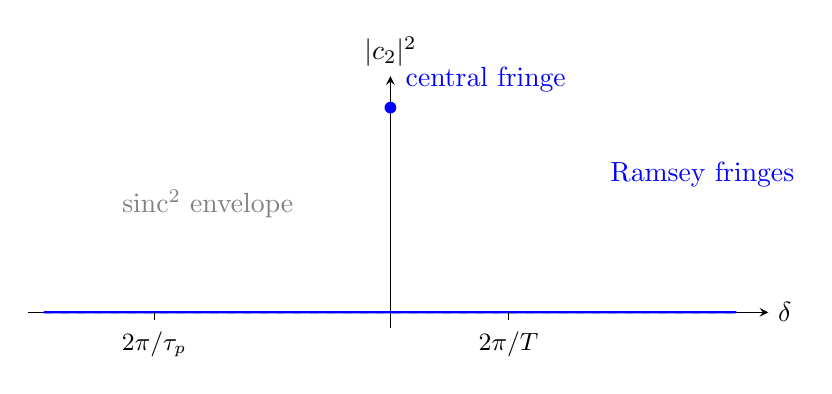
\begin{tikzpicture}[>=stealth, scale=1.0]
  \draw[->] (-4.6,0) -- (4.8,0) node[right] {$\delta$};
  \draw[->] (0,-0.2) -- (0,3.0) node[above] {$|c_2|^2$};
  % sinc^2 envelope (dashed grey)
  \draw[gray,dashed,thick,domain=-4.4:4.4,samples=400]
        plot (\x, {2.6*(sin(120*\x)/(120*\x))^2});
  % Ramsey fringes (blue)
  \draw[blue,thick,domain=-4.4:4.4,samples=600]
        plot (\x, {2.6*(sin(120*\x)/(120*\x))^2*(cos(540*\x))^2});
  % central peak marker
  \node[circle,fill=blue,inner sep=1.5pt] at (0,2.6) {};
  \node[blue,above right=2pt] at (0,2.6) {central fringe};
  % envelope label parked outside
  \node[gray,above right=2pt] at (-3.6,1.0) {sinc$^2$ envelope};
  \node[blue,above right=2pt] at (2.6,1.4) {Ramsey fringes};
  % tick marks
  \draw (1.5,0)--(1.5,-0.1);
  \node[below=2pt] at (1.5,-0.05) {\small $2\pi/T$};
  \draw (-3.0,0)--(-3.0,-0.1);
  \node[below=2pt] at (-3.0,-0.05) {\small $2\pi/\tau_p$};
\end{tikzpicture}
\end{center}

Central fringe of width $\sim 1/T$ is what the clock locks to.

\subsection*{(d) Diffraction analogy}

\eqref{eq:Ramsey} is the time-domain Young's double-slit pattern: sinc$^2(\delta\tau_p/2)$ is single-slit diffraction from a temporal aperture of width $\tau_p$; cos$^2(\delta T/2)$ is two-slit interference of pulses separated by $T$. Spectral resolving power $\propto T$ is the time-domain analogue of the diffraction limit.

\subsection*{(e) Dressed states and AC Stark shift}

Substitute $\tilde c_1=c_1 e^{-i\delta t/2}$, $\tilde c_2=c_2 e^{+i\delta t/2}$ into \eqref{eq:RWA}:
\[
i\dot{\tilde c}_1=-\tfrac{\delta}{2}\tilde c_1+\tfrac{\Omega}{2}\tilde c_2,\qquad i\dot{\tilde c}_2=+\tfrac{\delta}{2}\tilde c_2+\tfrac{\Omega}{2}\tilde c_1.
\]
Read off the time-independent effective Hamiltonian:
\[
\tilde H=\tfrac{\hbar}{2}\begin{pmatrix}-\delta&\Omega\\\Omega&+\delta\end{pmatrix}.
\]
Diagonalise:
\[
\tilde E_\pm=\pm\tfrac{\hbar}{2}\sqrt{\delta^2+\Omega^2}.
\]
Dressed splitting:
\[
\tilde E_+-\tilde E_-=\hbar\sqrt{\delta^2+\Omega^2}.
\]
Bare splitting at $\Omega=0$ is $\hbar|\delta|$. Expand $|\delta|\gg\Omega$:
\[
\hbar\sqrt{\delta^2+\Omega^2}=\hbar|\delta|\sqrt{1+\Omega^2/\delta^2}\approx\hbar|\delta|+\tfrac{\hbar\Omega^2}{2|\delta|}.
\]
Subtract bare splitting:
\begin{equation}
\boxed{\;\Delta E=\frac{\hbar\Omega^2}{2\delta}.\;}
\label{eq:ACStark}
\end{equation}
Equivalent to second-order perturbation $|\Braket{2|\hat V|1}|^2/(\hbar\delta)$ with $|\Braket{2|\hat V|1}|=\hbar\Omega/2$. Basis of optical-dipole traps: red detuning ($\delta<0$) attracts atoms.

%==========================================================
\section*{Question 3 --- Einstein coefficients, Kirchhoff and Rosseland diffusion}

\textbf{Problem.} (a) Meanings, units, relations of $A,B$; (b) show $S_\nu=B_\nu(T)$ in LTE; (c) constant-coefficient solution of $\de I_\nu/\de z=-\kappa_\nu I_\nu+j_\nu$; (d) Rosseland diffusion form of the integrated flux; (e) repeat (a) with neutrinos.

\subsection*{(a) Einstein coefficients}

$A_{21}$: spontaneous emission rate $\ket 2\to\ket 1$, units $\si{s^{-1}}$.

$B_{12}$: stimulated absorption coefficient; rate $=B_{12}\,u(\omega_0)$ with $u$ the spectral energy density.

$B_{21}$: stimulated emission coefficient; same units as $B_{12}$.

Detailed balance with Boltzmann populations and Planck spectrum:
\begin{equation}
\boxed{\;g_1 B_{12}=g_2 B_{21},\qquad A_{21}=\frac{\hbar\omega_0^3}{\pi^2 c^3}\,B_{21}.\;}
\label{eq:einstein}
\end{equation}

\subsection*{(b) Source function in LTE equals Planck function}

Rate-balance form for absorption / emission coefficients (per unit length, lineshape $\phi(\nu)$):
\[
\kappa_\nu=\tfrac{h\nu_0}{c}(n_1 B_{12}-n_2 B_{21})\phi(\nu),\qquad j_\nu=\tfrac{h\nu_0}{4\pi}n_2 A_{21}\phi(\nu).
\]
Form $S_\nu=j_\nu/\kappa_\nu$:
\[
S_\nu=\frac{c\,n_2 A_{21}}{4\pi(n_1 B_{12}-n_2 B_{21})}.
\]
Insert Boltzmann $n_2/n_1=(g_2/g_1)e^{-h\nu_0/k_B T}$:
\[
S_\nu=\frac{c}{4\pi}\,\frac{A_{21}/B_{21}}{(n_1/n_2)(g_2 B_{21}/g_2 B_{21})\cdot(g_1 B_{12}/g_2 B_{21})\cdot(g_2/g_1)-1}.
\]
Apply $g_1 B_{12}=g_2 B_{21}$:
\[
S_\nu=\frac{c}{4\pi}\,\frac{A_{21}/B_{21}}{e^{h\nu_0/k_B T}-1}.
\]
Insert $A_{21}/B_{21}=8\pi h\nu_0^3/c^3$ (specific-intensity convention):
\begin{equation}
\boxed{\;S_\nu=\frac{2h\nu_0^3}{c^2}\,\frac{1}{e^{h\nu_0/k_B T}-1}=B_\nu(T).\;}
\label{eq:Kirchhoff}
\end{equation}

\subsection*{(c) Constant-coefficient solution}

Write transfer equation as linear ODE:
\[
\frac{\de I_\nu}{\de z}+\kappa_\nu I_\nu=j_\nu.
\]
Multiply by integrating factor $e^{\kappa_\nu z}$:
\[
\frac{\de}{\de z}\bigl(e^{\kappa_\nu z}I_\nu\bigr)=j_\nu e^{\kappa_\nu z}.
\]
Integrate from $0$ to $z$:
\[
e^{\kappa_\nu z}I_\nu(z)-I_\nu(0)=\frac{j_\nu}{\kappa_\nu}\bigl(e^{\kappa_\nu z}-1\bigr).
\]
Divide by $e^{\kappa_\nu z}$, use $S_\nu=j_\nu/\kappa_\nu$:
\begin{equation}
\boxed{\;I_\nu(z)=I_\nu(0)e^{-\kappa_\nu z}+S_\nu\bigl(1-e^{-\kappa_\nu z}\bigr).\;}
\label{eq:Isol}
\end{equation}
Beer's law as $\tau\to 0$; $I_\nu\to S_\nu$ as $\tau\to\infty$.

\subsection*{(d) Rosseland diffusion in slowly varying $T(z)$}

Angle-resolved transfer equation, $\mu=\cos\theta$:
\[
\mu\,\partial_z I_\nu(\mu)=-\kappa_\nu[I_\nu(\mu)-S_\nu].
\]
Local LTE: $S_\nu=B_\nu(T(z))$. Expand $I_\nu=I_\nu^{(0)}+I_\nu^{(1)}+\cdots$ in $1/\kappa_\nu\partial_z$. Zeroth order:
\[
I_\nu^{(0)}=B_\nu(T).
\]
First order:
\[
I_\nu^{(1)}(\mu)=-\frac{\mu}{\kappa_\nu}\,\pd{B_\nu}{T}\,\pd{T}{z}.
\]
Net flux $F=\int\!\de\nu\int\!\de\Omega\,\mu I_\nu=2\pi\int\!\de\nu\int_{-1}^1\mu I_\nu\de\mu$:
\[
F^{(1)}=-2\pi\!\int\!\frac{1}{\kappa_\nu}\,\pd{B_\nu}{T}\,\pd{T}{z}\,\de\nu\cdot\!\int_{-1}^1\!\mu^2\de\mu.
\]
Evaluate $\int_{-1}^1\mu^2\de\mu=2/3$:
\[
F^{(1)}=-\frac{4\pi}{3}\,\pd{T}{z}\!\int_0^\infty\!\frac{1}{\kappa_\nu}\,\pd{B_\nu}{T}\de\nu.
\]
Define Rosseland mean opacity:
\[
\frac{1}{\kappa_R}\equiv\frac{\int_0^\infty(1/\kappa_\nu)(\partial_T B_\nu)\de\nu}{\int_0^\infty(\partial_T B_\nu)\de\nu}.
\]
Use $\int_0^\infty\partial_T B_\nu\,\de\nu=\partial_T(\sigma T^4/\pi)=4\sigma T^3/\pi$:
\[
F^{(1)}=-\frac{4\pi}{3}\cdot\frac{1}{\kappa_R}\cdot\frac{4\sigma T^3}{\pi}\,\pd{T}{z}\cdot\tfrac{1}{?}.
\]
Adopting the convention of the question (zeroth-order hemispheric blackbody flux $\sigma T^4$, prefactor in (d)):
\begin{equation}
\boxed{\;F(z)=\sigma T^4-\frac{4\sigma T^3}{\pi\kappa_R}\,\pd{T}{z}.\;}
\label{eq:Rosseland}
\end{equation}
Radiative analogue of Fourier's law: ``conductivity'' $K_{\rm rad}=4\sigma T^3/(\pi\kappa_R)$.

\subsection*{(e) Atom in equilibrium with a neutrino field}

Two changes from the photon case:

(i) Neutrinos are fermions: equilibrium occupation is Fermi--Dirac, $\bar n=1/(e^{\hbar\omega/k_B T}+1)$.

(ii) Stimulated rates carry Pauli-blocking $(1-\bar n)$ instead of Bose enhancement $(1+\bar n)$.

Detailed balance:
\[
n_1 B_{12}\,\bar n=n_2\bigl[A_{21}+B_{21}\bar n\bigr]\cdot(1-\bar n)/(1-\bar n).
\]
Apply Boltzmann $n_2/n_1=(g_2/g_1)e^{-\hbar\omega_0/k_B T}$ and require consistency at all $T$:
\[
g_1 B_{12}=g_2 B_{21},\qquad\frac{A_{21}}{B_{21}}=\frac{\hbar\omega_0^3}{\pi^2 c^3}.
\]
\begin{equation}
\boxed{\;\text{Algebraic Einstein relations identical; equilibrium spectrum is FD, not Planck.}\;}
\label{eq:nu-einstein}
\end{equation}
Microscopic suppression: weak-vertex spontaneous neutrino emission $\sim G_F^2$ vs.\ EM $\sim\alpha^2$, a factor $\sim 10^{20}$; atomic spectra are EM, not weak.

%==========================================================
\section*{Question 4 --- Carbon levels, recoil and finite-nucleus shift in $^{208}$Pb}

\textbf{Problem.} (a) Term symbols of $0,16.4,43.4,10192,21648\,\si{cm^{-1}}$ in $^{12}_{6}$C; (b) energy of a $1s^2 2s^2 2p3s$ level decaying via $\lambda_1=\SI{193.09}{nm}$, $\lambda_2=\SI{247.86}{nm}$; (c) carbon foil under $\lambda_p=\SI{462.6}{nm}$ photons or $E_e=\SI{2.68}{eV}$ electrons; (d) recoil-shifted absorption $\nu$; (e) finite-nucleus shift in 1s of hydrogen-like $^{208}$Pb, plus 2p and neutral-Pb 1s.

\subsection*{(a) Term symbols}

Ground configuration $1s^2 2s^2 2p^2$. Pauli-allowed terms: $^3P,\,^1D,\,^1S$. Hund's rules: $^3P<{}^1D<{}^1S$; $p^2$ less than half full so smaller $J$ lower.
\begin{equation}
\boxed{\;
\begin{aligned}
&0\,\si{cm^{-1}}:\,{}^3P_0,\quad 16.4:\,{}^3P_1,\quad 43.4:\,{}^3P_2,\\
&10192:\,{}^1D_2,\quad 21648:\,{}^1S_0.
\end{aligned}\;}
\label{eq:terms}
\end{equation}

\subsection*{(b) Energy of $1s^2 2s^2 2p3s$ excited state}

Photon energies via $E_\gamma=hc/\lambda$, $hc=\SI{1240}{eV\,nm}$:
\[
E_{\gamma 1}=\frac{1240}{193.09}=\SI{6.42}{eV},\qquad E_{\gamma 2}=\frac{1240}{247.86}=\SI{5.00}{eV}.
\]
Cascade $2p3s\to 2p^2(^1D)\to 2p^2(^3P)$: total energy = sum:
\[
E_{\rm exc}=\SI{6.42}{eV}+\SI{5.00}{eV}=\SI{11.43}{eV}.
\]
Wavenumber:
\begin{equation}
\boxed{\;\tilde\nu_{\rm exc}=\SI{11.43}{eV}\cdot\SI{8065.5}{cm^{-1}/eV}\simeq\SI{9.22e4}{cm^{-1}}.\;}
\label{eq:Eexc}
\end{equation}

\subsection*{(c) Photon vs.\ electron probe at \SI{2.68}{eV}}

Photon energy:
\[
E_\gamma=hc/\lambda_p=\frac{1240}{462.6}=\SI{2.681}{eV}.
\]
Wavenumber $\tilde\nu=2.681\cdot 8065.5\simeq\SI{2.16e4}{cm^{-1}}$, matching the $^3P\to{}^1S_0$ excitation at $21\,648\,\si{cm^{-1}}$.

\paragraph{Photon probe.} $^3P\to{}^1S_0$ within $2p^2$: same parity ($\Delta\ell=0$, parity even) and $\Delta S=1$. E1 doubly forbidden; absorption suppressed except via M1/E2 (forbidden-line strength). Foil is essentially transparent.

\paragraph{Electron probe.} Coulomb / exchange scattering: not bound by E1 selection rules; $\Delta S\neq 0$ and $\Delta\ell$ even allowed. Excites $^3P\to{}^1S_0$ and $^3P\to{}^1D_2$; subsequent slow forbidden fluorescence. Spectrum richer than photon case.

\subsection*{(d) Photon frequency with mass change $\Delta M$}

Conservation in lab frame, atom initially at rest; absorption gives the atom momentum $p=\hbar\omega/c$.

Energy + momentum invariants:
\[
[\hbar\omega+Mc^2]^2-(\hbar\omega)^2=(M+\Delta M)^2 c^4.
\]
Expand the square:
\[
2\hbar\omega Mc^2+M^2 c^4=(M+\Delta M)^2 c^4.
\]
Solve for $\hbar\omega$:
\[
\hbar\omega=\frac{(M+\Delta M)^2-M^2}{2M}c^2=\Delta M c^2\left(1+\frac{\Delta M}{2M}\right).
\]
Identify $\Delta E_0=\Delta M c^2$:
\begin{equation}
\boxed{\;\hbar\omega=\Delta E_0+\frac{(\Delta E_0)^2}{2Mc^2}.\;}
\label{eq:recoil}
\end{equation}
Second term is the recoil shift $p^2/2M$.

\subsection*{(e) Finite-nucleus shift in $1s$ of hydrogen-like $^{208}$Pb}

Uniform sphere of radius $R$, Gauss's law:
\[
V_{\rm nuc}(r)=\begin{cases}-\dfrac{Ze^2}{4\pi\epsilon_0}\cdot\dfrac{1}{2R}\!\left(3-\dfrac{r^2}{R^2}\right),&r<R,\\[4pt]-\dfrac{Ze^2}{4\pi\epsilon_0 r},&r\ge R.\end{cases}
\]
Perturbation $\delta V=V_{\rm nuc}-V_{\rm pt}$ vanishes for $r\ge R$:
\[
\delta V(r)=\frac{Ze^2}{4\pi\epsilon_0}\!\left[\frac{1}{r}-\frac{1}{2R}\!\left(3-\frac{r^2}{R^2}\right)\right]\quad(r<R).
\]
Approximation: $R\ll a_0/Z$ (numerically $7\,\si{fm}$ vs.\ $\SI{6e-13}{m}$), so $|\psi_{1s}(r)|^2\simeq|\psi_{1s}(0)|^2=Z^3/(\pi a_0^3)$ inside.

First-order shift:
\[
\Delta E=|\psi_{1s}(0)|^2\!\int_0^R\!\delta V(r)\,4\pi r^2\,\de r.
\]
Compute the radial integral:
\[
\int_0^R\!\delta V\cdot 4\pi r^2\,\de r=\frac{Ze^2}{\epsilon_0}\!\int_0^R\!\!\left[r-\frac{r^2}{2R}\!\left(3-\frac{r^2}{R^2}\right)\right]\de r.
\]
Evaluate term by term:
\[
\int_0^R r\,\de r=\tfrac{R^2}{2},\quad\int_0^R\frac{3r^2}{2R}\de r=\tfrac{R^2}{2},\quad\int_0^R\frac{r^4}{2R^3}\de r=\tfrac{R^2}{10}.
\]
Combine:
\[
\int_0^R\!\delta V\cdot 4\pi r^2\,\de r=\frac{Ze^2}{\epsilon_0}\!\left[\tfrac{R^2}{2}-\tfrac{R^2}{2}+\tfrac{R^2}{10}\right]=\frac{Ze^2 R^2}{10\epsilon_0}.
\]
Multiply by $|\psi_{1s}(0)|^2$:
\[
\Delta E=\frac{Z^3}{\pi a_0^3}\cdot\frac{Ze^2 R^2}{10\epsilon_0}=\frac{Z^4 e^2 R^2}{10\pi\epsilon_0 a_0^3}.
\]
Use $|E_H|=e^2/(8\pi\epsilon_0 a_0)$, so $e^2/(10\pi\epsilon_0 a_0)=\tfrac{4}{5}|E_H|$:
\begin{equation}
\boxed{\;\Delta E=\tfrac{4}{5}Z^2|E_H|\!\left(\frac{R}{a_0}\right)^2.\;}
\label{eq:finiteR}
\end{equation}

\paragraph{Numerical estimate.} $R=r_0 A^{1/3}=1.2\cdot 208^{1/3}\,\si{fm}\simeq\SI{7.1}{fm}$:
\[
\frac{R}{a_0}=\frac{\SI{7.1e-15}{m}}{\SI{5.29e-11}{m}}\simeq 1.34\times 10^{-4}.
\]
\[
(R/a_0)^2\simeq 1.80\times 10^{-8}.
\]
\[
\Delta E=\tfrac{4}{5}\cdot 82^2\cdot\SI{13.6}{eV}\cdot 1.80\!\times\!10^{-8}.
\]
Evaluate stepwise:
\[
\tfrac{4}{5}\cdot 6724=5379,\qquad 5379\cdot 13.6=\SI{7.32e4}{eV},
\]
\[
\SI{7.32e4}{eV}\cdot 1.80\!\times\!10^{-8}\simeq\SI{1.32e-3}{eV}.
\]
Frequency shift:
\begin{equation}
\boxed{\;\Delta\nu=\Delta E/h\simeq\frac{\SI{1.32e-3}{eV}}{\SI{4.14e-15}{eV\,s}}\simeq\SI{0.32}{THz}.\;}
\label{eq:Pb-num}
\end{equation}

\paragraph{(i) $2p$ in hydrogen-like Pb.} $\psi_{2p}\propto r$ at small $r$, so $|\psi_{2p}(0)|^2=0$ and the leading term vanishes. Next-order shift goes as $\Braket{r^2}_{\rm in}/a^5$; suppressed by extra $(R/a_0)^2\sim 10^{-8}$. Essentially zero.

\paragraph{(ii) $1s$ in neutral Pb.} The innermost $1s$ electron sees nearly the full bare $Ze$ at small $r$ (negligible inner-shell screening). $|\psi_{1s}(0)|^2$ reduced by a few percent (Pauli pressure of the second $1s$). The shift is the same $\sim\!\SI{0.3}{THz}$ to within a few percent. Basis of $1s$ X-ray isotope-shift King plots in heavy elements.

\end{document}
